\documentclass[twoside]{book}

% Packages required by doxygen
\usepackage{fixltx2e}
\usepackage{calc}
\usepackage{doxygen}
\usepackage[export]{adjustbox} % also loads graphicx
\usepackage{graphicx}
\usepackage[utf8]{inputenc}
\usepackage{makeidx}
\usepackage{multicol}
\usepackage{multirow}
\PassOptionsToPackage{warn}{textcomp}
\usepackage{textcomp}
\usepackage[nointegrals]{wasysym}
\usepackage[table]{xcolor}

% Font selection
\usepackage[T1]{fontenc}
\usepackage[scaled=.90]{helvet}
\usepackage{courier}
\usepackage{amssymb}
\usepackage{sectsty}
\renewcommand{\familydefault}{\sfdefault}
\allsectionsfont{%
  \fontseries{bc}\selectfont%
  \color{darkgray}%
}
\renewcommand{\DoxyLabelFont}{%
  \fontseries{bc}\selectfont%
  \color{darkgray}%
}
\newcommand{\+}{\discretionary{\mbox{\scriptsize$\hookleftarrow$}}{}{}}

% Page & text layout
\usepackage{geometry}
\geometry{%
  a4paper,%
  top=2.5cm,%
  bottom=2.5cm,%
  left=2.5cm,%
  right=2.5cm%
}
\tolerance=750
\hfuzz=15pt
\hbadness=750
\setlength{\emergencystretch}{15pt}
\setlength{\parindent}{0cm}
\setlength{\parskip}{3ex plus 2ex minus 2ex}
\makeatletter
\renewcommand{\paragraph}{%
  \@startsection{paragraph}{4}{0ex}{-1.0ex}{1.0ex}{%
    \normalfont\normalsize\bfseries\SS@parafont%
  }%
}
\renewcommand{\subparagraph}{%
  \@startsection{subparagraph}{5}{0ex}{-1.0ex}{1.0ex}{%
    \normalfont\normalsize\bfseries\SS@subparafont%
  }%
}
\makeatother

% Headers & footers
\usepackage{fancyhdr}
\pagestyle{fancyplain}
\fancyhead[LE]{\fancyplain{}{\bfseries\thepage}}
\fancyhead[CE]{\fancyplain{}{}}
\fancyhead[RE]{\fancyplain{}{\bfseries\leftmark}}
\fancyhead[LO]{\fancyplain{}{\bfseries\rightmark}}
\fancyhead[CO]{\fancyplain{}{}}
\fancyhead[RO]{\fancyplain{}{\bfseries\thepage}}
\fancyfoot[LE]{\fancyplain{}{}}
\fancyfoot[CE]{\fancyplain{}{}}
\fancyfoot[RE]{\fancyplain{}{\bfseries\scriptsize Generated by Doxygen }}
\fancyfoot[LO]{\fancyplain{}{\bfseries\scriptsize Generated by Doxygen }}
\fancyfoot[CO]{\fancyplain{}{}}
\fancyfoot[RO]{\fancyplain{}{}}
\renewcommand{\footrulewidth}{0.4pt}
\renewcommand{\chaptermark}[1]{%
  \markboth{#1}{}%
}
\renewcommand{\sectionmark}[1]{%
  \markright{\thesection\ #1}%
}

% Indices & bibliography
\usepackage{natbib}
\usepackage[titles]{tocloft}
\setcounter{tocdepth}{3}
\setcounter{secnumdepth}{5}
\makeindex

% Hyperlinks (required, but should be loaded last)
\usepackage{ifpdf}
\ifpdf
  \usepackage[pdftex,pagebackref=true]{hyperref}
\else
  \usepackage[ps2pdf,pagebackref=true]{hyperref}
\fi
\hypersetup{%
  colorlinks=true,%
  linkcolor=blue,%
  citecolor=blue,%
  unicode%
}

% Custom commands
\newcommand{\clearemptydoublepage}{%
  \newpage{\pagestyle{empty}\cleardoublepage}%
}

\usepackage{caption}
\captionsetup{labelsep=space,justification=centering,font={bf},singlelinecheck=off,skip=4pt,position=top}

%===== C O N T E N T S =====

\begin{document}

% Titlepage & ToC
\hypersetup{pageanchor=false,
             bookmarksnumbered=true,
             pdfencoding=unicode
            }
\pagenumbering{roman}
\begin{titlepage}
\vspace*{7cm}
\begin{center}%
{\Large Lu\+Animator }\\
\vspace*{1cm}
{\large Generated by Doxygen 1.8.11}\\
\end{center}
\end{titlepage}
\clearemptydoublepage
\tableofcontents
\clearemptydoublepage
\pagenumbering{arabic}
\hypersetup{pageanchor=true}

%--- Begin generated contents ---
\chapter{Namespace Index}
\section{Packages}
Here are the packages with brief descriptions (if available)\+:\begin{DoxyCompactList}
\item\contentsline{section}{\hyperlink{namespace_drawables_generator_tool}{Drawables\+Generator\+Tool} }{\pageref{namespace_drawables_generator_tool}}{}
\item\contentsline{section}{\hyperlink{namespace_lu_animator_v2}{Lu\+Animator\+V2} }{\pageref{namespace_lu_animator_v2}}{}
\item\contentsline{section}{\hyperlink{namespace_star_cheat_reloaded}{Star\+Cheat\+Reloaded} }{\pageref{namespace_star_cheat_reloaded}}{}
\item\contentsline{section}{\hyperlink{namespace_star_cheat_reloaded_1_1_g_u_i}{Star\+Cheat\+Reloaded.\+G\+UI} }{\pageref{namespace_star_cheat_reloaded_1_1_g_u_i}}{}
\end{DoxyCompactList}

\chapter{Hierarchical Index}
\section{Class Hierarchy}
This inheritance list is sorted roughly, but not completely, alphabetically\+:\begin{DoxyCompactList}
\item \contentsline{section}{Star\+Cheat\+Reloaded.\+G\+U\+I.\+Directive}{\pageref{class_star_cheat_reloaded_1_1_g_u_i_1_1_directive}}{}
\item \contentsline{section}{Lu\+Animator\+V2.\+emote\+Node}{\pageref{class_lu_animator_v2_1_1emote_node}}{}
\item \contentsline{section}{Lu\+Animator\+V2.\+File\+Generator}{\pageref{class_lu_animator_v2_1_1_file_generator}}{}
\item \contentsline{section}{Lu\+Animator\+V2.\+mode\+Node}{\pageref{class_lu_animator_v2_1_1mode_node}}{}
\item User\+Control\begin{DoxyCompactList}
\item \contentsline{section}{Lu\+Animator\+V2.\+Border\+Background}{\pageref{class_lu_animator_v2_1_1_border_background}}{}
\end{DoxyCompactList}
\item Window\begin{DoxyCompactList}
\item \contentsline{section}{Lu\+Animator\+V2.\+About\+Window}{\pageref{class_lu_animator_v2_1_1_about_window}}{}
\item \contentsline{section}{Lu\+Animator\+V2.\+Crop\+Window}{\pageref{class_lu_animator_v2_1_1_crop_window}}{}
\item \contentsline{section}{Lu\+Animator\+V2.\+Main\+Window}{\pageref{class_lu_animator_v2_1_1_main_window}}{}
\item \contentsline{section}{Lu\+Animator\+V2.\+Progress\+Bar\+Task\+On\+Ui\+Thread}{\pageref{class_lu_animator_v2_1_1_progress_bar_task_on_ui_thread}}{}
\end{DoxyCompactList}
\item Application\begin{DoxyCompactList}
\item \contentsline{section}{Lu\+Animator\+V2.\+App}{\pageref{class_lu_animator_v2_1_1_app}}{}
\end{DoxyCompactList}
\end{DoxyCompactList}

\chapter{Class Index}
\section{Class List}
Here are the classes, structs, unions and interfaces with brief descriptions\+:\begin{DoxyCompactList}
\item\contentsline{section}{\hyperlink{class_lu_animator_v2_1_1_about_window}{Lu\+Animator\+V2.\+About\+Window} \\*Interaction logic for \hyperlink{class_lu_animator_v2_1_1_about_window}{About\+Window} }{\pageref{class_lu_animator_v2_1_1_about_window}}{}
\item\contentsline{section}{\hyperlink{class_lu_animator_v2_1_1_app}{Lu\+Animator\+V2.\+App} \\*Interaction logic for App.\+xaml }{\pageref{class_lu_animator_v2_1_1_app}}{}
\item\contentsline{section}{\hyperlink{class_lu_animator_v2_1_1_border_background}{Lu\+Animator\+V2.\+Border\+Background} \\*Interaction logic for Border\+Background.\+xaml }{\pageref{class_lu_animator_v2_1_1_border_background}}{}
\item\contentsline{section}{\hyperlink{class_lu_animator_v2_1_1_crop_window}{Lu\+Animator\+V2.\+Crop\+Window} \\*Interaction logic for Crop\+Window.\+xaml }{\pageref{class_lu_animator_v2_1_1_crop_window}}{}
\item\contentsline{section}{\hyperlink{class_star_cheat_reloaded_1_1_g_u_i_1_1_directive}{Star\+Cheat\+Reloaded.\+G\+U\+I.\+Directive} }{\pageref{class_star_cheat_reloaded_1_1_g_u_i_1_1_directive}}{}
\item\contentsline{section}{\hyperlink{class_lu_animator_v2_1_1emote_node}{Lu\+Animator\+V2.\+emote\+Node} }{\pageref{class_lu_animator_v2_1_1emote_node}}{}
\item\contentsline{section}{\hyperlink{class_lu_animator_v2_1_1_file_generator}{Lu\+Animator\+V2.\+File\+Generator} \\*Saves and loads the luanimation projects }{\pageref{class_lu_animator_v2_1_1_file_generator}}{}
\item\contentsline{section}{\hyperlink{class_lu_animator_v2_1_1_main_window}{Lu\+Animator\+V2.\+Main\+Window} \\*Interaction logic for Main\+Window.\+xaml }{\pageref{class_lu_animator_v2_1_1_main_window}}{}
\item\contentsline{section}{\hyperlink{class_lu_animator_v2_1_1mode_node}{Lu\+Animator\+V2.\+mode\+Node} }{\pageref{class_lu_animator_v2_1_1mode_node}}{}
\item\contentsline{section}{\hyperlink{class_lu_animator_v2_1_1_progress_bar_task_on_ui_thread}{Lu\+Animator\+V2.\+Progress\+Bar\+Task\+On\+Ui\+Thread} }{\pageref{class_lu_animator_v2_1_1_progress_bar_task_on_ui_thread}}{}
\end{DoxyCompactList}

\chapter{Namespace Documentation}
\hypertarget{namespace_drawables_generator_tool}{}\section{Drawables\+Generator\+Tool Namespace Reference}
\label{namespace_drawables_generator_tool}\index{Drawables\+Generator\+Tool@{Drawables\+Generator\+Tool}}
\subsection*{Classes}
\begin{DoxyCompactItemize}
\item 
class {\bfseries Drawable\+Utilities}
\end{DoxyCompactItemize}

\hypertarget{namespace_lu_animator_v2}{}\section{Lu\+Animator\+V2 Namespace Reference}
\label{namespace_lu_animator_v2}\index{Lu\+Animator\+V2@{Lu\+Animator\+V2}}
\subsection*{Classes}
\begin{DoxyCompactItemize}
\item 
class \hyperlink{class_lu_animator_v2_1_1_about_window}{About\+Window}
\begin{DoxyCompactList}\small\item\em Interaction logic for \hyperlink{class_lu_animator_v2_1_1_about_window}{About\+Window} \end{DoxyCompactList}\item 
class \hyperlink{class_lu_animator_v2_1_1_app}{App}
\begin{DoxyCompactList}\small\item\em Interaction logic for App.\+xaml \end{DoxyCompactList}\item 
class {\bfseries Bitmap\+Converter}
\begin{DoxyCompactList}\small\item\em Converter between Bitmap and Bitmap\+Source/$>$ \end{DoxyCompactList}\item 
class \hyperlink{class_lu_animator_v2_1_1_border_background}{Border\+Background}
\begin{DoxyCompactList}\small\item\em Interaction logic for Border\+Background.\+xaml \end{DoxyCompactList}\item 
class \hyperlink{class_lu_animator_v2_1_1_crop_window}{Crop\+Window}
\begin{DoxyCompactList}\small\item\em Interaction logic for Crop\+Window.\+xaml \end{DoxyCompactList}\item 
class \hyperlink{class_lu_animator_v2_1_1emote_node}{emote\+Node}
\item 
class \hyperlink{class_lu_animator_v2_1_1_file_generator}{File\+Generator}
\begin{DoxyCompactList}\small\item\em Saves and loads the luanimation projects \end{DoxyCompactList}\item 
class {\bfseries Image\+Cropper}
\item 
class \hyperlink{class_lu_animator_v2_1_1_main_window}{Main\+Window}
\begin{DoxyCompactList}\small\item\em Interaction logic for Main\+Window.\+xaml \end{DoxyCompactList}\item 
class \hyperlink{class_lu_animator_v2_1_1mode_node}{mode\+Node}
\item 
class \hyperlink{class_lu_animator_v2_1_1_progress_bar_task_on_ui_thread}{Progress\+Bar\+Task\+On\+Ui\+Thread}
\end{DoxyCompactItemize}

\hypertarget{namespace_star_cheat_reloaded}{}\section{Star\+Cheat\+Reloaded Namespace Reference}
\label{namespace_star_cheat_reloaded}\index{Star\+Cheat\+Reloaded@{Star\+Cheat\+Reloaded}}
\subsection*{Namespaces}
\begin{DoxyCompactItemize}
\end{DoxyCompactItemize}

\hypertarget{namespace_star_cheat_reloaded_1_1_g_u_i}{}\section{Star\+Cheat\+Reloaded.\+G\+UI Namespace Reference}
\label{namespace_star_cheat_reloaded_1_1_g_u_i}\index{Star\+Cheat\+Reloaded.\+G\+UI@{Star\+Cheat\+Reloaded.\+G\+UI}}
\subsection*{Classes}
\begin{DoxyCompactItemize}
\item 
class \hyperlink{class_star_cheat_reloaded_1_1_g_u_i_1_1_directive}{Directive}
\end{DoxyCompactItemize}

\chapter{Class Documentation}
\hypertarget{class_lu_animator_v2_1_1_about_window}{}\section{Lu\+Animator\+V2.\+About\+Window Class Reference}
\label{class_lu_animator_v2_1_1_about_window}\index{Lu\+Animator\+V2.\+About\+Window@{Lu\+Animator\+V2.\+About\+Window}}


Interaction logic for \hyperlink{class_lu_animator_v2_1_1_about_window}{About\+Window}  


Inheritance diagram for Lu\+Animator\+V2.\+About\+Window\+:\begin{figure}[H]
\begin{center}
\leavevmode
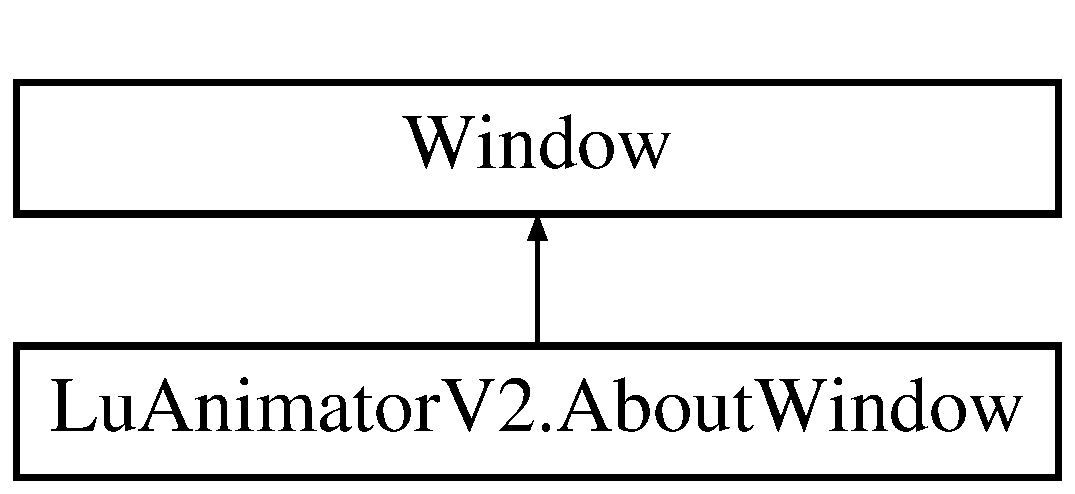
\includegraphics[height=2.000000cm]{class_lu_animator_v2_1_1_about_window}
\end{center}
\end{figure}


\subsection{Detailed Description}
Interaction logic for \hyperlink{class_lu_animator_v2_1_1_about_window}{About\+Window} 



The documentation for this class was generated from the following file\+:\begin{DoxyCompactItemize}
\item 
C\+:/\+Users/\+Degranon/\+Desktop/Программы/\+Lu\+Animator-\/backup/\+Lu\+Animator\+V2/About.\+xaml.\+cs\end{DoxyCompactItemize}

\hypertarget{class_lu_animator_v2_1_1_app}{}\section{Lu\+Animator\+V2.\+App Class Reference}
\label{class_lu_animator_v2_1_1_app}\index{Lu\+Animator\+V2.\+App@{Lu\+Animator\+V2.\+App}}


Interaction logic for App.\+xaml  


Inheritance diagram for Lu\+Animator\+V2.\+App\+:\begin{figure}[H]
\begin{center}
\leavevmode
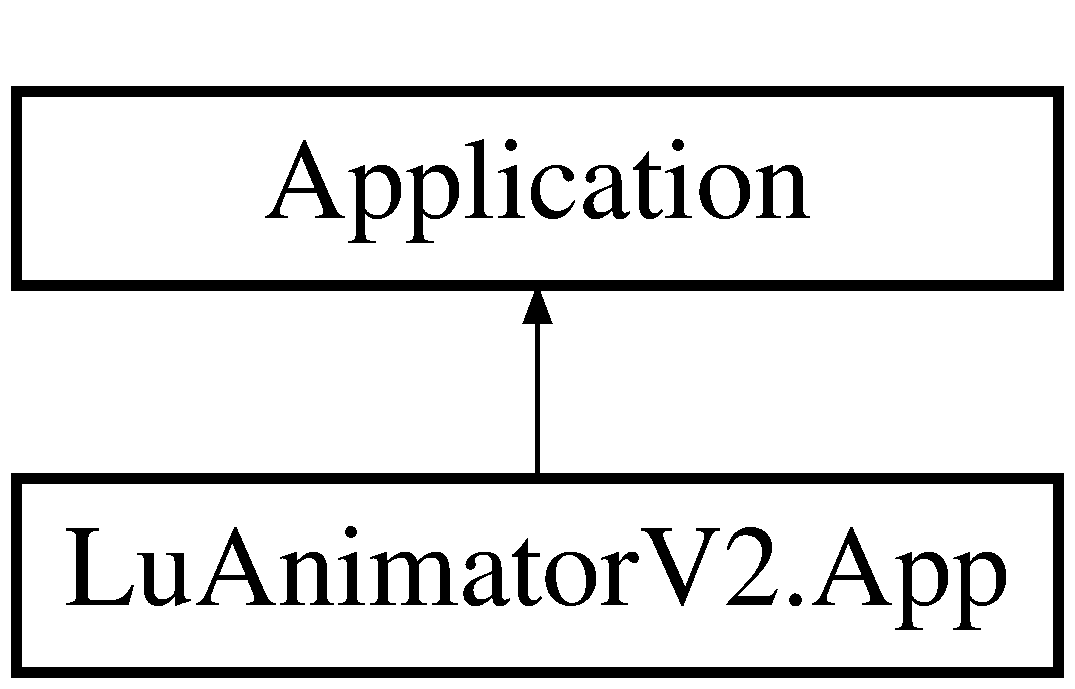
\includegraphics[height=2.000000cm]{class_lu_animator_v2_1_1_app}
\end{center}
\end{figure}


\subsection{Detailed Description}
Interaction logic for App.\+xaml 



The documentation for this class was generated from the following file\+:\begin{DoxyCompactItemize}
\item 
C\+:/\+Users/\+Degranon/\+Desktop/Программы/\+Lu\+Animator-\/backup/\+Lu\+Animator\+V2/App.\+xaml.\+cs\end{DoxyCompactItemize}

\hypertarget{class_lu_animator_v2_1_1_border_background}{}\section{Lu\+Animator\+V2.\+Border\+Background Class Reference}
\label{class_lu_animator_v2_1_1_border_background}\index{Lu\+Animator\+V2.\+Border\+Background@{Lu\+Animator\+V2.\+Border\+Background}}


Interaction logic for Border\+Background.\+xaml  


Inheritance diagram for Lu\+Animator\+V2.\+Border\+Background\+:\begin{figure}[H]
\begin{center}
\leavevmode
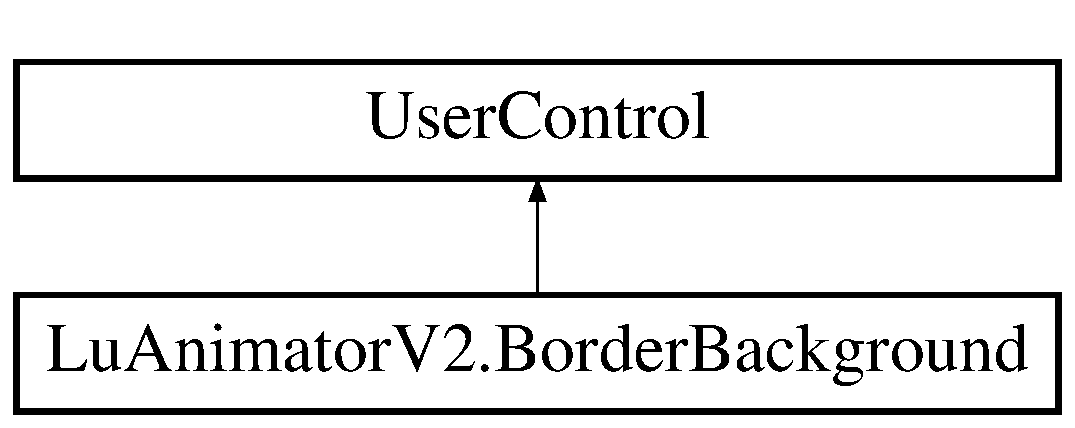
\includegraphics[height=2.000000cm]{class_lu_animator_v2_1_1_border_background}
\end{center}
\end{figure}


\subsection{Detailed Description}
Interaction logic for Border\+Background.\+xaml 



The documentation for this class was generated from the following file\+:\begin{DoxyCompactItemize}
\item 
C\+:/\+Users/\+Degranon/\+Desktop/Программы/\+Lu\+Animator-\/backup/\+Lu\+Animator\+V2/Border\+Background.\+xaml.\+cs\end{DoxyCompactItemize}

\hypertarget{class_lu_animator_v2_1_1_crop_window}{}\section{Lu\+Animator\+V2.\+Crop\+Window Class Reference}
\label{class_lu_animator_v2_1_1_crop_window}\index{Lu\+Animator\+V2.\+Crop\+Window@{Lu\+Animator\+V2.\+Crop\+Window}}


Interaction logic for Crop\+Window.\+xaml  


Inheritance diagram for Lu\+Animator\+V2.\+Crop\+Window\+:\begin{figure}[H]
\begin{center}
\leavevmode
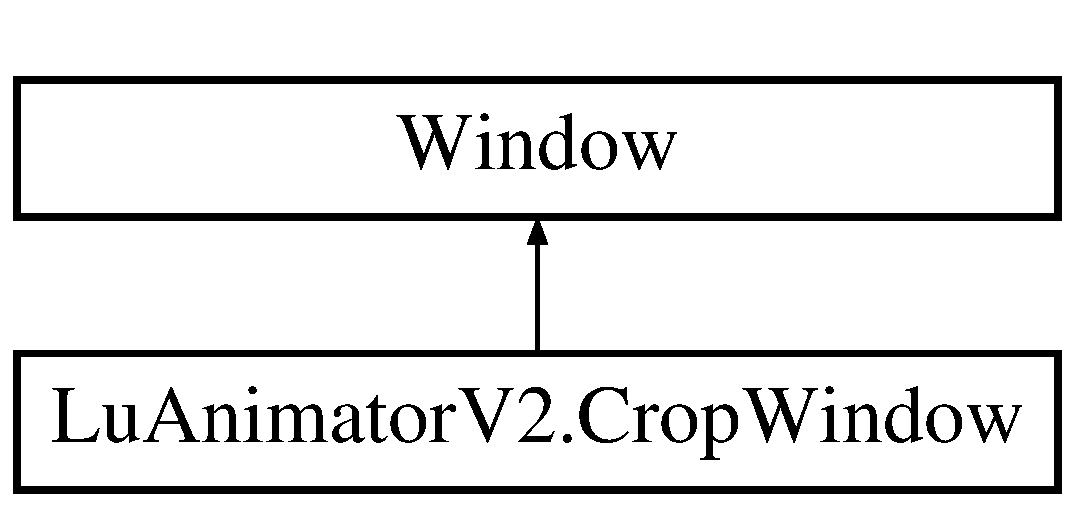
\includegraphics[height=2.000000cm]{class_lu_animator_v2_1_1_crop_window}
\end{center}
\end{figure}


\subsection{Detailed Description}
Interaction logic for Crop\+Window.\+xaml 



The documentation for this class was generated from the following file\+:\begin{DoxyCompactItemize}
\item 
C\+:/\+Users/\+Degranon/\+Desktop/Программы/\+Lu\+Animator-\/backup/\+Lu\+Animator\+V2/Crop\+Window.\+xaml.\+cs\end{DoxyCompactItemize}

\hypertarget{class_star_cheat_reloaded_1_1_g_u_i_1_1_directive}{}\section{Star\+Cheat\+Reloaded.\+G\+U\+I.\+Directive Class Reference}
\label{class_star_cheat_reloaded_1_1_g_u_i_1_1_directive}\index{Star\+Cheat\+Reloaded.\+G\+U\+I.\+Directive@{Star\+Cheat\+Reloaded.\+G\+U\+I.\+Directive}}
\subsection*{Public Member Functions}
\begin{DoxyCompactItemize}
\item 
{\bfseries Directive} (string type, params string\mbox{[}$\,$\mbox{]} parameters)\hypertarget{class_star_cheat_reloaded_1_1_g_u_i_1_1_directive_ad0205c669cfc7ccab78c5a7eca2a7fc7}{}\label{class_star_cheat_reloaded_1_1_g_u_i_1_1_directive_ad0205c669cfc7ccab78c5a7eca2a7fc7}

\item 
{\bfseries Directive} (string directive)\hypertarget{class_star_cheat_reloaded_1_1_g_u_i_1_1_directive_acb69c455a559c22b652d6504bb923147}{}\label{class_star_cheat_reloaded_1_1_g_u_i_1_1_directive_acb69c455a559c22b652d6504bb923147}

\item 
override string {\bfseries To\+String} ()\hypertarget{class_star_cheat_reloaded_1_1_g_u_i_1_1_directive_adee74ec55176ec4b8a2453fda72f1415}{}\label{class_star_cheat_reloaded_1_1_g_u_i_1_1_directive_adee74ec55176ec4b8a2453fda72f1415}

\item 
{\bfseries Directive} (string directive, bool skip\+First\+Char)\hypertarget{class_star_cheat_reloaded_1_1_g_u_i_1_1_directive_a7cecd5d34a0c81bd85536e5733d168db}{}\label{class_star_cheat_reloaded_1_1_g_u_i_1_1_directive_a7cecd5d34a0c81bd85536e5733d168db}

\end{DoxyCompactItemize}
\subsection*{Static Public Member Functions}
\begin{DoxyCompactItemize}
\item 
static void {\bfseries Apply\+Directives} (ref Bitmap b, string directives)\hypertarget{class_star_cheat_reloaded_1_1_g_u_i_1_1_directive_a7331903b152cd55abda0961aabefbf91}{}\label{class_star_cheat_reloaded_1_1_g_u_i_1_1_directive_a7331903b152cd55abda0961aabefbf91}

\item 
static void {\bfseries Apply\+Directives} (Graphics g, ref Bitmap b, string directives)\hypertarget{class_star_cheat_reloaded_1_1_g_u_i_1_1_directive_a5a91ea5df9d586890808cbc6412becbc}{}\label{class_star_cheat_reloaded_1_1_g_u_i_1_1_directive_a5a91ea5df9d586890808cbc6412becbc}

\item 
static void {\bfseries Apply\+Directives} (ref Bitmap b, string\mbox{[}$\,$\mbox{]} directives)\hypertarget{class_star_cheat_reloaded_1_1_g_u_i_1_1_directive_a2bead4c75d80d3fafb41e4c336f7cae6}{}\label{class_star_cheat_reloaded_1_1_g_u_i_1_1_directive_a2bead4c75d80d3fafb41e4c336f7cae6}

\item 
static void {\bfseries Apply\+Directives} (Graphics g, ref Bitmap b, string\mbox{[}$\,$\mbox{]} directives)\hypertarget{class_star_cheat_reloaded_1_1_g_u_i_1_1_directive_aa03b3c725f03f3649922d87b07127acb}{}\label{class_star_cheat_reloaded_1_1_g_u_i_1_1_directive_aa03b3c725f03f3649922d87b07127acb}

\end{DoxyCompactItemize}
\subsection*{Properties}
\begin{DoxyCompactItemize}
\item 
string {\bfseries Type}\hspace{0.3cm}{\ttfamily  \mbox{[}get, set\mbox{]}}\hypertarget{class_star_cheat_reloaded_1_1_g_u_i_1_1_directive_a4f235e66648a94f42739b8723324e942}{}\label{class_star_cheat_reloaded_1_1_g_u_i_1_1_directive_a4f235e66648a94f42739b8723324e942}

\item 
string\mbox{[}$\,$\mbox{]} {\bfseries Parameters} = null\hspace{0.3cm}{\ttfamily  \mbox{[}get, set\mbox{]}}\hypertarget{class_star_cheat_reloaded_1_1_g_u_i_1_1_directive_a04b3d2d22a2450471b78564c7e874a90}{}\label{class_star_cheat_reloaded_1_1_g_u_i_1_1_directive_a04b3d2d22a2450471b78564c7e874a90}

\end{DoxyCompactItemize}


The documentation for this class was generated from the following file\+:\begin{DoxyCompactItemize}
\item 
C\+:/\+Users/\+Degranon/\+Desktop/Программы/\+Lu\+Animator-\/backup/\+Lu\+Animator\+V2/Directive.\+cs\end{DoxyCompactItemize}

\hypertarget{class_lu_animator_v2_1_1emote_node}{}\section{Lu\+Animator\+V2.\+emote\+Node Class Reference}
\label{class_lu_animator_v2_1_1emote_node}\index{Lu\+Animator\+V2.\+emote\+Node@{Lu\+Animator\+V2.\+emote\+Node}}
\subsection*{Public Attributes}
\begin{DoxyCompactItemize}
\item 
string {\bfseries name}\hypertarget{class_lu_animator_v2_1_1emote_node_a731deded5be04d85bf0f186e7b07c34e}{}\label{class_lu_animator_v2_1_1emote_node_a731deded5be04d85bf0f186e7b07c34e}

\item 
int {\bfseries speed}\hypertarget{class_lu_animator_v2_1_1emote_node_ac766a2bfc7c4d1afa86bcdf53c35895b}{}\label{class_lu_animator_v2_1_1emote_node_ac766a2bfc7c4d1afa86bcdf53c35895b}

\item 
bool {\bfseries looping}\hypertarget{class_lu_animator_v2_1_1emote_node_a75774a71bedb73f8aa9066e590ec541a}{}\label{class_lu_animator_v2_1_1emote_node_a75774a71bedb73f8aa9066e590ec541a}

\item 
Bitmap\+Source\mbox{[}$\,$\mbox{]} {\bfseries frames}\hypertarget{class_lu_animator_v2_1_1emote_node_ae39e90d5edf3da2ed5b5a1729cae3435}{}\label{class_lu_animator_v2_1_1emote_node_ae39e90d5edf3da2ed5b5a1729cae3435}

\item 
Bitmap\+Source\mbox{[}$\,$\mbox{]} {\bfseries fullbright\+Frames}\hypertarget{class_lu_animator_v2_1_1emote_node_ad43278045af59da24d62bdb1c5b034bf}{}\label{class_lu_animator_v2_1_1emote_node_ad43278045af59da24d62bdb1c5b034bf}

\item 
string\mbox{[}$\,$\mbox{]} {\bfseries sound} = null\hypertarget{class_lu_animator_v2_1_1emote_node_afa10dfc82a4d37acb974f1819d4bc7a8}{}\label{class_lu_animator_v2_1_1emote_node_afa10dfc82a4d37acb974f1819d4bc7a8}

\item 
bool {\bfseries sound\+Loop}\hypertarget{class_lu_animator_v2_1_1emote_node_a2eccbac74421c46877f1e72797f838a4}{}\label{class_lu_animator_v2_1_1emote_node_a2eccbac74421c46877f1e72797f838a4}

\item 
double {\bfseries sound\+Interval}\hypertarget{class_lu_animator_v2_1_1emote_node_a85d34354ad778f8986aa1ca31453e63e}{}\label{class_lu_animator_v2_1_1emote_node_a85d34354ad778f8986aa1ca31453e63e}

\item 
double {\bfseries sound\+Volume} = 1\hypertarget{class_lu_animator_v2_1_1emote_node_a1c7b5201794826c4d7741086446d7d3b}{}\label{class_lu_animator_v2_1_1emote_node_a1c7b5201794826c4d7741086446d7d3b}

\item 
double {\bfseries sound\+Pitch} = 1\hypertarget{class_lu_animator_v2_1_1emote_node_a1930b66a157861ad383c451cd2087d02}{}\label{class_lu_animator_v2_1_1emote_node_a1930b66a157861ad383c451cd2087d02}

\end{DoxyCompactItemize}


The documentation for this class was generated from the following file\+:\begin{DoxyCompactItemize}
\item 
C\+:/\+Users/\+Degranon/\+Desktop/Программы/\+Lu\+Animator-\/backup/\+Lu\+Animator\+V2/emote\+Node.\+cs\end{DoxyCompactItemize}

\hypertarget{class_lu_animator_v2_1_1_file_generator}{}\section{Lu\+Animator\+V2.\+File\+Generator Class Reference}
\label{class_lu_animator_v2_1_1_file_generator}\index{Lu\+Animator\+V2.\+File\+Generator@{Lu\+Animator\+V2.\+File\+Generator}}


Saves and loads the luanimation projects  


\subsection*{Static Public Member Functions}
\begin{DoxyCompactItemize}
\item 
static string \hyperlink{class_lu_animator_v2_1_1_file_generator_abffd6182cb6ba1f037209693b2639466}{To\+Json} (Animation\+Collection animation\+Collection)
\begin{DoxyCompactList}\small\item\em Create Json object by the animation collection \end{DoxyCompactList}\item 
static Animation\+Collection \hyperlink{class_lu_animator_v2_1_1_file_generator_a1b842faa7436ec1b4238429c7340764f}{To\+Animation\+Collection} (string path)
\begin{DoxyCompactList}\small\item\em Generates the \end{DoxyCompactList}\end{DoxyCompactItemize}
\subsection*{Static Protected Member Functions}
\begin{DoxyCompactItemize}
\item 
static string \hyperlink{class_lu_animator_v2_1_1_file_generator_a2a6e42c8ff1f6d09f9caa6dd8e325c08}{Generate\+Directive} (Bitmap\+Source bsource)
\begin{DoxyCompactList}\small\item\em Generate the starbound single texture directive by the given frame \end{DoxyCompactList}\end{DoxyCompactItemize}


\subsection{Detailed Description}
Saves and loads the luanimation projects 



\subsection{Member Function Documentation}
\index{Lu\+Animator\+V2\+::\+File\+Generator@{Lu\+Animator\+V2\+::\+File\+Generator}!Generate\+Directive@{Generate\+Directive}}
\index{Generate\+Directive@{Generate\+Directive}!Lu\+Animator\+V2\+::\+File\+Generator@{Lu\+Animator\+V2\+::\+File\+Generator}}
\subsubsection[{\texorpdfstring{Generate\+Directive(\+Bitmap\+Source bsource)}{GenerateDirective(BitmapSource bsource)}}]{\setlength{\rightskip}{0pt plus 5cm}static string Lu\+Animator\+V2.\+File\+Generator.\+Generate\+Directive (
\begin{DoxyParamCaption}
\item[{Bitmap\+Source}]{bsource}
\end{DoxyParamCaption}
)\hspace{0.3cm}{\ttfamily [static]}, {\ttfamily [protected]}}\hypertarget{class_lu_animator_v2_1_1_file_generator_a2a6e42c8ff1f6d09f9caa6dd8e325c08}{}\label{class_lu_animator_v2_1_1_file_generator_a2a6e42c8ff1f6d09f9caa6dd8e325c08}


Generate the starbound single texture directive by the given frame 


\begin{DoxyParams}{Parameters}
{\em bsource} & A frame to create directives from\\
\hline
\end{DoxyParams}
\begin{DoxyReturn}{Returns}
The directive string
\end{DoxyReturn}
\index{Lu\+Animator\+V2\+::\+File\+Generator@{Lu\+Animator\+V2\+::\+File\+Generator}!To\+Animation\+Collection@{To\+Animation\+Collection}}
\index{To\+Animation\+Collection@{To\+Animation\+Collection}!Lu\+Animator\+V2\+::\+File\+Generator@{Lu\+Animator\+V2\+::\+File\+Generator}}
\subsubsection[{\texorpdfstring{To\+Animation\+Collection(string path)}{ToAnimationCollection(string path)}}]{\setlength{\rightskip}{0pt plus 5cm}static Animation\+Collection Lu\+Animator\+V2.\+File\+Generator.\+To\+Animation\+Collection (
\begin{DoxyParamCaption}
\item[{string}]{path}
\end{DoxyParamCaption}
)\hspace{0.3cm}{\ttfamily [static]}}\hypertarget{class_lu_animator_v2_1_1_file_generator_a1b842faa7436ec1b4238429c7340764f}{}\label{class_lu_animator_v2_1_1_file_generator_a1b842faa7436ec1b4238429c7340764f}


Generates the 


\begin{DoxyParams}{Parameters}
{\em path} & \\
\hline
\end{DoxyParams}
\begin{DoxyReturn}{Returns}

\end{DoxyReturn}
\index{Lu\+Animator\+V2\+::\+File\+Generator@{Lu\+Animator\+V2\+::\+File\+Generator}!To\+Json@{To\+Json}}
\index{To\+Json@{To\+Json}!Lu\+Animator\+V2\+::\+File\+Generator@{Lu\+Animator\+V2\+::\+File\+Generator}}
\subsubsection[{\texorpdfstring{To\+Json(\+Animation\+Collection animation\+Collection)}{ToJson(AnimationCollection animationCollection)}}]{\setlength{\rightskip}{0pt plus 5cm}static string Lu\+Animator\+V2.\+File\+Generator.\+To\+Json (
\begin{DoxyParamCaption}
\item[{Animation\+Collection}]{animation\+Collection}
\end{DoxyParamCaption}
)\hspace{0.3cm}{\ttfamily [static]}}\hypertarget{class_lu_animator_v2_1_1_file_generator_abffd6182cb6ba1f037209693b2639466}{}\label{class_lu_animator_v2_1_1_file_generator_abffd6182cb6ba1f037209693b2639466}


Create Json object by the animation collection 


\begin{DoxyParams}{Parameters}
{\em animation\+Collection} & Animation\\
\hline
\end{DoxyParams}
\begin{DoxyReturn}{Returns}
Json containing line, ready to be saved
\end{DoxyReturn}


The documentation for this class was generated from the following file\+:\begin{DoxyCompactItemize}
\item 
C\+:/\+Users/\+Degranon/\+Desktop/Программы/\+Lu\+Animator-\/backup/\+Lu\+Animator\+V2/File\+Generator.\+cs\end{DoxyCompactItemize}

\hypertarget{class_lu_animator_v2_1_1_main_window}{}\section{Lu\+Animator\+V2.\+Main\+Window Class Reference}
\label{class_lu_animator_v2_1_1_main_window}\index{Lu\+Animator\+V2.\+Main\+Window@{Lu\+Animator\+V2.\+Main\+Window}}


Interaction logic for Main\+Window.\+xaml  


Inheritance diagram for Lu\+Animator\+V2.\+Main\+Window\+:\begin{figure}[H]
\begin{center}
\leavevmode
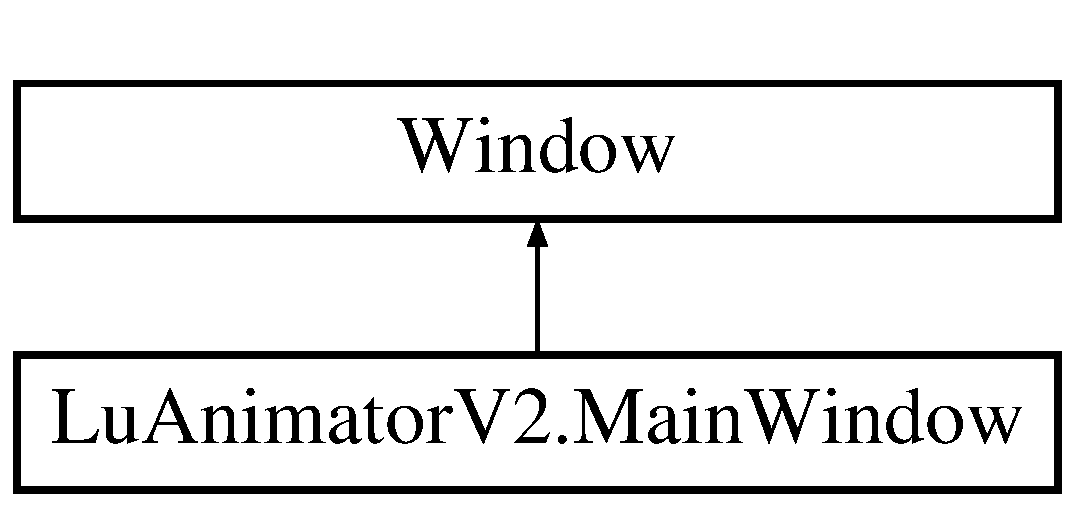
\includegraphics[height=2.000000cm]{class_lu_animator_v2_1_1_main_window}
\end{center}
\end{figure}
\subsection*{Public Member Functions}
\begin{DoxyCompactItemize}
\item 
void \hyperlink{class_lu_animator_v2_1_1_main_window_a24f05f16c39805c58885169377a3817b}{Open\+\_\+\+Click} (object sender, Routed\+Event\+Args e)
\begin{DoxyCompactList}\small\item\em A handler for Open File menu option \end{DoxyCompactList}\end{DoxyCompactItemize}
\subsection*{Static Public Member Functions}
\begin{DoxyCompactItemize}
\item 
static bool \hyperlink{class_lu_animator_v2_1_1_main_window_aeb67233dd3b8a17a1365881c637c9b10}{Is\+Valid\+Image} (string path)
\begin{DoxyCompactList}\small\item\em Returns whether the given path is a valid image \end{DoxyCompactList}\end{DoxyCompactItemize}
\subsection*{Protected Member Functions}
\begin{DoxyCompactItemize}
\item 
void \hyperlink{class_lu_animator_v2_1_1_main_window_ae88c0edde1914c9afb01b27fb59ee8f9}{Window\+\_\+\+Closing} (object sender, System.\+Component\+Model.\+Cancel\+Event\+Args e)
\begin{DoxyCompactList}\small\item\em Ask user to save his project before exiting the application \end{DoxyCompactList}\end{DoxyCompactItemize}


\subsection{Detailed Description}
Interaction logic for Main\+Window.\+xaml 



\subsection{Member Function Documentation}
\index{Lu\+Animator\+V2\+::\+Main\+Window@{Lu\+Animator\+V2\+::\+Main\+Window}!Is\+Valid\+Image@{Is\+Valid\+Image}}
\index{Is\+Valid\+Image@{Is\+Valid\+Image}!Lu\+Animator\+V2\+::\+Main\+Window@{Lu\+Animator\+V2\+::\+Main\+Window}}
\subsubsection[{\texorpdfstring{Is\+Valid\+Image(string path)}{IsValidImage(string path)}}]{\setlength{\rightskip}{0pt plus 5cm}static bool Lu\+Animator\+V2.\+Main\+Window.\+Is\+Valid\+Image (
\begin{DoxyParamCaption}
\item[{string}]{path}
\end{DoxyParamCaption}
)\hspace{0.3cm}{\ttfamily [static]}}\hypertarget{class_lu_animator_v2_1_1_main_window_aeb67233dd3b8a17a1365881c637c9b10}{}\label{class_lu_animator_v2_1_1_main_window_aeb67233dd3b8a17a1365881c637c9b10}


Returns whether the given path is a valid image 


\begin{DoxyParams}{Parameters}
{\em path} & The path to check for validity\\
\hline
\end{DoxyParams}
\begin{DoxyReturn}{Returns}
True if the given string is an image.
\end{DoxyReturn}
\index{Lu\+Animator\+V2\+::\+Main\+Window@{Lu\+Animator\+V2\+::\+Main\+Window}!Open\+\_\+\+Click@{Open\+\_\+\+Click}}
\index{Open\+\_\+\+Click@{Open\+\_\+\+Click}!Lu\+Animator\+V2\+::\+Main\+Window@{Lu\+Animator\+V2\+::\+Main\+Window}}
\subsubsection[{\texorpdfstring{Open\+\_\+\+Click(object sender, Routed\+Event\+Args e)}{Open_Click(object sender, RoutedEventArgs e)}}]{\setlength{\rightskip}{0pt plus 5cm}void Lu\+Animator\+V2.\+Main\+Window.\+Open\+\_\+\+Click (
\begin{DoxyParamCaption}
\item[{object}]{sender, }
\item[{Routed\+Event\+Args}]{e}
\end{DoxyParamCaption}
)}\hypertarget{class_lu_animator_v2_1_1_main_window_a24f05f16c39805c58885169377a3817b}{}\label{class_lu_animator_v2_1_1_main_window_a24f05f16c39805c58885169377a3817b}


A handler for Open File menu option 


\begin{DoxyParams}{Parameters}
{\em sender} & The source of the event\\
\hline
{\em e} & The Routed\+Event\+Args instance containing the event data.\\
\hline
\end{DoxyParams}
\index{Lu\+Animator\+V2\+::\+Main\+Window@{Lu\+Animator\+V2\+::\+Main\+Window}!Window\+\_\+\+Closing@{Window\+\_\+\+Closing}}
\index{Window\+\_\+\+Closing@{Window\+\_\+\+Closing}!Lu\+Animator\+V2\+::\+Main\+Window@{Lu\+Animator\+V2\+::\+Main\+Window}}
\subsubsection[{\texorpdfstring{Window\+\_\+\+Closing(object sender, System.\+Component\+Model.\+Cancel\+Event\+Args e)}{Window_Closing(object sender, System.ComponentModel.CancelEventArgs e)}}]{\setlength{\rightskip}{0pt plus 5cm}void Lu\+Animator\+V2.\+Main\+Window.\+Window\+\_\+\+Closing (
\begin{DoxyParamCaption}
\item[{object}]{sender, }
\item[{System.\+Component\+Model.\+Cancel\+Event\+Args}]{e}
\end{DoxyParamCaption}
)\hspace{0.3cm}{\ttfamily [protected]}}\hypertarget{class_lu_animator_v2_1_1_main_window_ae88c0edde1914c9afb01b27fb59ee8f9}{}\label{class_lu_animator_v2_1_1_main_window_ae88c0edde1914c9afb01b27fb59ee8f9}


Ask user to save his project before exiting the application 


\begin{DoxyParams}{Parameters}
{\em sender} & The source of the event\\
\hline
{\em e} & The System.\+Component\+Model.\+Cancel\+Event\+Args instance containing the event data.\\
\hline
\end{DoxyParams}


The documentation for this class was generated from the following file\+:\begin{DoxyCompactItemize}
\item 
C\+:/\+Users/\+Degranon/\+Desktop/Программы/\+Lu\+Animator-\/backup/\+Lu\+Animator\+V2/Main\+Window.\+xaml.\+cs\end{DoxyCompactItemize}

\hypertarget{class_lu_animator_v2_1_1mode_node}{}\section{Lu\+Animator\+V2.\+mode\+Node Class Reference}
\label{class_lu_animator_v2_1_1mode_node}\index{Lu\+Animator\+V2.\+mode\+Node@{Lu\+Animator\+V2.\+mode\+Node}}
\subsection*{Public Attributes}
\begin{DoxyCompactItemize}
\item 
string {\bfseries mode\+Name}\hypertarget{class_lu_animator_v2_1_1mode_node_ad6d9fbc8b54fe2e9adf33823af11133e}{}\label{class_lu_animator_v2_1_1mode_node_ad6d9fbc8b54fe2e9adf33823af11133e}

\item 
bool {\bfseries invisible}\hypertarget{class_lu_animator_v2_1_1mode_node_a8d1bb4d6dc5155ad46bd90f75a766f4a}{}\label{class_lu_animator_v2_1_1mode_node_a8d1bb4d6dc5155ad46bd90f75a766f4a}

\item 
int {\bfseries xtranslation}\hypertarget{class_lu_animator_v2_1_1mode_node_a480e0753baf433225980dc8b7338d7cd}{}\label{class_lu_animator_v2_1_1mode_node_a480e0753baf433225980dc8b7338d7cd}

\item 
int {\bfseries ytranslation}\hypertarget{class_lu_animator_v2_1_1mode_node_ab15a6d98a49a72484598769b8925c299}{}\label{class_lu_animator_v2_1_1mode_node_ab15a6d98a49a72484598769b8925c299}

\item 
double {\bfseries framescale}\hypertarget{class_lu_animator_v2_1_1mode_node_a3e8cb94b7f2c3d851f7d8ea1d804b6e5}{}\label{class_lu_animator_v2_1_1mode_node_a3e8cb94b7f2c3d851f7d8ea1d804b6e5}

\item 
List$<$ \hyperlink{class_lu_animator_v2_1_1emote_node}{emote\+Node} $>$ {\bfseries emotes}\hypertarget{class_lu_animator_v2_1_1mode_node_acf3d6e7f0a8ed4a09b755672cc7c2689}{}\label{class_lu_animator_v2_1_1mode_node_acf3d6e7f0a8ed4a09b755672cc7c2689}

\end{DoxyCompactItemize}


The documentation for this class was generated from the following file\+:\begin{DoxyCompactItemize}
\item 
C\+:/\+Users/\+Degranon/\+Desktop/Программы/\+Lu\+Animator-\/backup/\+Lu\+Animator\+V2/mode\+Node.\+cs\end{DoxyCompactItemize}

\hypertarget{class_lu_animator_v2_1_1_progress_bar_task_on_ui_thread}{}\section{Lu\+Animator\+V2.\+Progress\+Bar\+Task\+On\+Ui\+Thread Class Reference}
\label{class_lu_animator_v2_1_1_progress_bar_task_on_ui_thread}\index{Lu\+Animator\+V2.\+Progress\+Bar\+Task\+On\+Ui\+Thread@{Lu\+Animator\+V2.\+Progress\+Bar\+Task\+On\+Ui\+Thread}}
Inheritance diagram for Lu\+Animator\+V2.\+Progress\+Bar\+Task\+On\+Ui\+Thread\+:\begin{figure}[H]
\begin{center}
\leavevmode
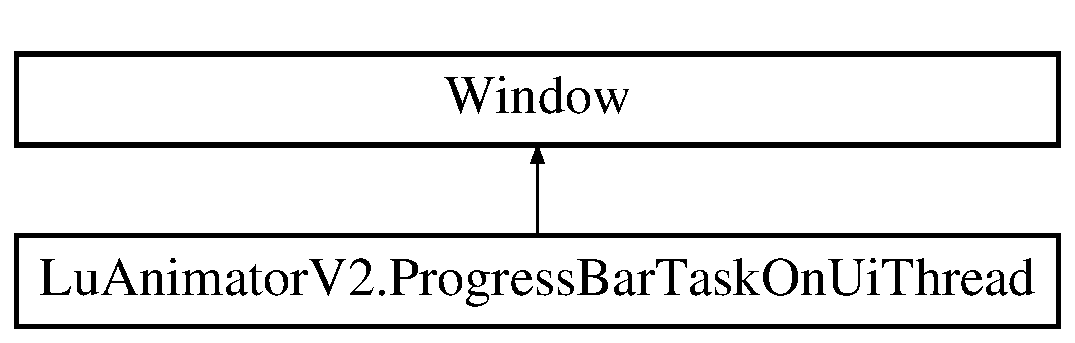
\includegraphics[height=2.000000cm]{class_lu_animator_v2_1_1_progress_bar_task_on_ui_thread}
\end{center}
\end{figure}
\subsection*{Public Member Functions}
\begin{DoxyCompactItemize}
\item 
{\bfseries Progress\+Bar\+Task\+On\+Ui\+Thread} (string title)\hypertarget{class_lu_animator_v2_1_1_progress_bar_task_on_ui_thread_a0baff16de01e84df95e3f60cadfc4723}{}\label{class_lu_animator_v2_1_1_progress_bar_task_on_ui_thread_a0baff16de01e84df95e3f60cadfc4723}

\end{DoxyCompactItemize}


The documentation for this class was generated from the following file\+:\begin{DoxyCompactItemize}
\item 
C\+:/\+Users/\+Degranon/\+Desktop/Программы/\+Lu\+Animator-\/backup/\+Lu\+Animator\+V2/waiting.\+xaml.\+cs\end{DoxyCompactItemize}

%--- End generated contents ---

% Index
\backmatter
\newpage
\phantomsection
\clearemptydoublepage
\addcontentsline{toc}{chapter}{Index}
\printindex

\end{document}
